\chapter{Bio-inspired optimization techniques}
\label{chap:bioalgorithms}

Optimization is the task of finding a solution to a problem that is better, or even the best compared to other solutions. A common optimization example is the traveling salesman problem (TSP) \cite{alexander2005history}. In TSP, a salesman needs to visit a set of cities that are connected to each other through paths of varying length. The goal is to find the shortest tour, such that the salesman visits each city exactly once and, at the end, returns to the city where he started the travel.

\section{Single objective optimization}
Optimization is generally done according to a defined goal, also called objective. In the TSP example, the objective is to find the shortest path for a complete tour. If there is just one objective the problem is called single objective optimization problem (SOP). 

\noindent\textbf{Definition (SOP)}: a SOP is defined by the pair $P=(S,f)$, where
\begin{itemize}
  \item $S$ is the set of possible solutions also called solution space or search space
  \item $f: \ S \mapsto {\rm I\!R}$ is the objective function that we want to minimize or maximize
\end{itemize}
The process of finding the global optimum is called global optimization. The global minimum optimization for the problem stated above is given in formula \eqref{eq:global-minimum-optimization}.

\begin{equation}\label{eq:global-minimum-optimization}
  s' \in S \ | \ (f(s') \leq f(s) \ \mbox{for all} \ s \in S)
\end{equation}

In words: we want to find a solution that is better than the other solutions in S.

\section{Multi objective optimization}
We talk about a multi objective optimization problem (MOP), if we have several conflicting objectives that we want to optimize at the same time. Non conflicting objectives can be combined which leads, in the case that no objective is in conflict with any other, to a SOP.

\noindent\textbf{Definition (MOP)}: a MOP is defined by $P=(\mathbf{S},\mathbf{F})$, where
\begin{itemize}
  \item $\mathbf{S}$ is a vector over the set of possible solutions also called solution space or search space
  \item $\mathbf{F} = (f_1,...,f_k): \ \mathbf{S} \mapsto {\rm I\!R^k}$ are the $k$ objective functions that we want to minimize or maximize
\end{itemize}

To optimize a MOP, a vector $\mathbf{x} = [x_1,...,x_k] \in S^k$ needs to be found which satisfies the $m$ inequality constraints $g_i(\mathbf{x}) \ge 0, i=1,...,m$, the p equality constrains $h_i(\mathbf{x}) = 0, i=1,...,p$ and minimizes (maximizes) the components of the vector function $\mathbf{F}$. It should be noted that $g_i(\mathbf{x}) \ge 0$ and $h_i(\mathbf{x}) = 0$ represent constraints that must be fulfilled while minimizing (or maximizing) $\mathbf{F}$.

% \noindent\textbf{Definition (MOP)}: a MOP is defined as finding a vector $\mathbf{x} = [x_1,...,x_n] \in \Omega$, which satisfies the $m$ inequality constraints $g_i(\mathbf{x}) \ge 0, i=1,...,m$, the p equality constrains $h_i(\mathbf{x}) = 0, i=1,...,p$ and minimizes (maximizes) the components of the vector function $\mathbf{F}(\mathbf{x}) = (f_1(\mathbf{x}), ..., f_k(\mathbf{x}))$, where $f_1,...,f_k$ are the $k$ objective functions. It should be noted that $g_i(\mathbf{x}) \ge 0$ and $h_i(\mathbf{x}) = 0$ represent constraints that must be fulfilled while minimizing (or maximizing) $\mathbf{F}(\mathbf{x})$. The universe $\Omega$ contains all possible $\mathbf{x}$ that can be used to satisfy an evaluation of $\mathbf{F}(\mathbf{x})$.

If we extend the TSP example, the two objectives are to find a) the shortest path, that b) costs as little as possible. The shortest path includes driving on the highway (causing higher costs due to toll fee), the cheapest path forces the salesman to drive on a normal street (longer distance). So we have to find a compromise between the two conflicting goals which means that there isn't a single best solution, but a set of solutions. Some solutions may result in a shorter path, where other ones may result in lower costs. When optimizing a MOP, the task is to find the set of solutions from which a decision maker (usually a human) selects the final solution.

It's not obvious how to compare two solutions in MOP. Figure \ref{fig:dominance} gives three examples of a problem with four objectives, in each example the solutions A and B are compared, the task is to minimize a problem. In figure \ref{fig:dominance}(a), solution A is better than solution B, as all values of A are smaller than their respective values in B. In figure \ref{fig:dominance}(b), B is better than A for the same reason. The situation in figure \ref{fig:dominance}(c) is more complicated and doesn't give a clear answer to the problem, as some values in A are smaller than their respective values in B and vice versa. One could now argue, that solution A is better than solution B, because there are more elements in A that are smaller with respect to their elements in B. But this does not hold true, as the number of smaller values does not say anything about the optimality of the solution. Considering the TSP example, what is a better solution, the distance or the gas consumption? This can not be answered in general and depends on the user preference at a given moment of time. To find a set of solutions for a MOP, the Pareto Optimality theory is used \cite{ehrgott2005multicriteria}.

\begin{figure}[ht!]
  \centering
  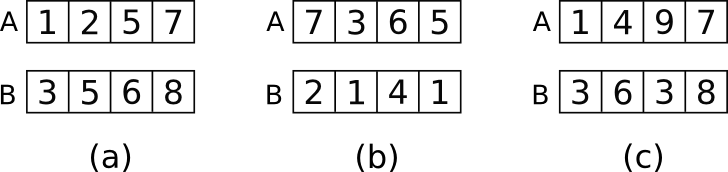
\includegraphics[width=100mm,natwidth=728,natheight=172]{bioinsp-dominance.png}
  \caption{Comparing solutions: (a) a is better than b, (b) b is better than a, (c) none is better - a and b are non-dominated}
  \label{fig:dominance}
\end{figure}

The Pareto Optimality theory defines the concept of Pareto Dominance, that can be used to compare two solutions. Figure \ref{fig:dominance2} gives an example of Pareto Dominance.

\begin{figure}[ht!]
  \centering
  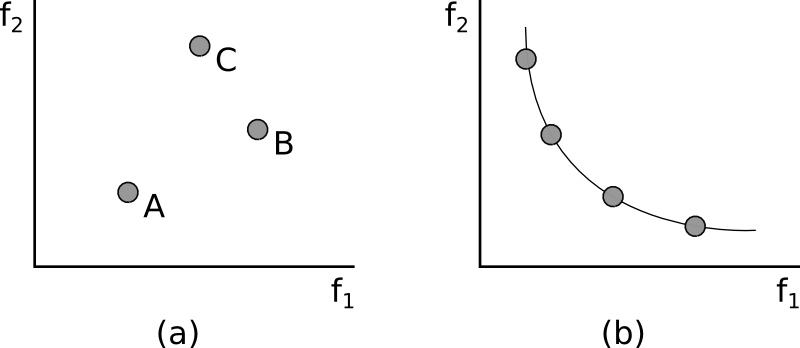
\includegraphics[width=110mm,natwidth=800,natheight=348]{bioinsp-dominance2.png}
  \caption{Pareto Dominance: (a) A dominates B and C, (b) all points are non-dominated}
  \label{fig:dominance2}
\end{figure}

\noindent\textbf{Definition (Pareto Dominance)}: a vector $\mathbf{u} = (u_1,...,u_k)$ is said to dominate a vector $\mathbf{v} = (v_1,...,v_k)$ (denoted by $\mathbf{u} \preceq \mathbf{v}$), if and only if $\mathbf{u}$ is partially less than $\mathbf{v}$, i.e., $\forall_i \in \{1,...,k\}, u_i \leq v_i \land \exists i \in \{1,...,k\}: u_i < v_i$.

In figure \ref{fig:dominance2}(a), we see that A dominates the solutions B and C, because
\begin{itemize}
  \item the values for $f_1$ and $f_2$ of A are the same or smaller than the corresponding values for B respectively C
  \item at least one of the values for A is smaller than the corresponding values for B respectively C
\end{itemize}
In figure \ref{fig:dominance2}(b) we see that no solution dominates another solution.

Using the concept of dominance, it is possible to define when a solution is optimal, this is known as Pareto Optimality.

\noindent\textbf{Definition (Pareto Optimality)}: a solution $\mathbf{x}$ is Pareto Optimal, if there is no $\mathbf{x'} \in \Omega$ for which $\mathbf{v} = \mathbf{F}(\mathbf{x'}) = (f_1(\mathbf{x'}),...,f_k(\mathbf{x'}))$ dominates $\mathbf{u} = \mathbf{F}(\mathbf{x}) = (f_1(\mathbf{x}),...,f_k(\mathbf{x}))$.

This means that no objective of a Pareto Optimal solution $\mathbf{x}$ can be improved without negatively affecting at least one of it's other objectives.

The solution to a MOP is then the set of non-dominated solutions, also called the Pareto Optimal Set.

\noindent\textbf{Definition (Pareto Optimal Set)}: for a given MOP $\mathbf{F}(\mathbf{x})$, the Pareto Optimal Set is defined as $\mathcal{P}^* = \{\mathbf{x} \in \Omega | \neg \exists \mathbf{x'} \in \Omega, \mathbf{F}(\mathbf{x'}) \preceq \mathbf{F}(\mathbf{x}) \}$

Its correspondence in the objective space (that is, the space where the results of the the objective functions lay) is called the Pareto Optimal Front, or just Pareto Front.

\noindent\textbf{Definition (Pareto Front)}: for a given MOP $\mathbf{F}(\mathbf{x})$ and Pareto Optimal Set $\mathcal{P}^*$, the Pareto Front $\mathcal{PF}^*$ is defined as $\mathcal{PF}^* = \{\mathbf{F}(\mathbf{x}) | \mathbf{x} \in \Omega \}$

When searching for the solutions of a MOP the goal is to find an approximation to the Pareto Front that:
\begin{itemize}
  \item has good convergence to the optimal Pareto Front, i.e. it is as near to the optimal Pareto Front as possible
  \item has good diversity, i.e. the solutions are well distributed throughout the Pareto Front
\end{itemize}

Figure \ref{fig:conv-div} gives an example for convergence and diversity of the Pareto Front. In figure \ref{fig:conv-div}(a) we have a Pareto Front with a bad convergence, as it is far away from the optimal/true Pareto Front. Figure \ref{fig:conv-div}(b) shows a Pareto Front that has bad divergence, i.e. several sections of the optimal Pareto Front are not covered with solutions. Figure \ref{fig:conv-div}(c) shows the ideal case, where the Pareto Front matches with the optimal Pareto Front - this is the desired solution.

\begin{figure}[ht!]
  \centering
  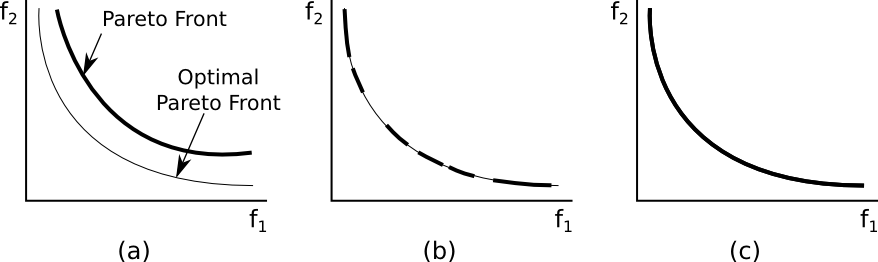
\includegraphics[width=130mm,natwidth=878,natheight=262]{bioinsp-conv-div.png}
  \caption{Example Pareto Fronts: (a) Pareto Front with bad convergence, (b) Pareto Front with bad divergence, (c) ideal case, where the Pareto Front matches the optimal Pareto Front}
  \label{fig:conv-div}
\end{figure}

\section{Complexity considerations}
Optimization is usually a computationally intensive task. For the TSP example, we can compute how many different solutions exist for a problem with $n$ cities, using formula \eqref{eq:tsp-cities}. Already a small number of cities entails a large number of solutions. For example, if we have 15 cities, we have a search space of over 43 billion solutions that we need to evaluate to get the best solution (assuming that we have no better suited technique to solve the problem). This number grows quickly if new cities are added and soon it becomes impossible to compute the optimal solution.

\begin{equation}\label{eq:tsp-cities}
  (n - 1)! / 2, \ \mbox{where} \ n \ \mbox{is the number of cities}
\end{equation}

Often there is no need to find the best solution to a problem, or there is no way at all. Instead it is sufficient to find a good enough solution in reasonable time. Approximation techniques can be used for this purpose. They don't guarantee to find the exact optimal solution, as they don't evaluate all solutions of the entire solution space. The advantage of approximation techniques is that they deliver solutions in a fast way. The results are usually near-optimal, although they can also be arbitrarily bad.

One well known family of approximation techniques are the metaheuristics \cite{yang2010nature}. A metaheuristic defines an abstract sequence of steps that leads to the optimization of a problem. As such, they are not problem specific and can be applied to a broad range of optimization problems.

\section{Optimization, inspired by nature}
Bio-inspired optimization techniques are a sub family of the metaheuristics. The name derives from the fact that they mimic behaviors observed in nature. For example, genetic algorithms (GA) \cite{sivanandam2008genetic} imitate the concept of evolution where only the fittest individuals survive and reproduce. Another example is particle swarm optimization (PSO) \cite{kennedy2010particle} that mimics the behavior of a flock of birds.

Bio-inspired optimization techniques are used today in many areas, like mechanical and electrical engineering, image processing, machine learning, network optimization, data mining etc. \cite{sivanandam2008genetic}.

\subsection{Genetic algorithm}
\label{chap:bioalgorithms:ga}
Genetic algorithms (GAs) are population-based optimization strategies. The population consists of $n$ individuals, each one representing a solution to the optimization problem. Every individual gets assigned a fitness value which represents its adoption to the environment. The fitness value is computed according to the optimization objective.

The idea behind genetic algorithms is to iteratively evolve the population towards individuals better adopted to the environment, which in an optimization problem means solutions of higher quality (preferably the optimum). The evolution is performed by applying selection, recombination and mutation to the population.

Recombination is performed by selecting two or more individuals out of the whole population. Those individuals are called the parent individuals. Fitter individuals are preferred for the recombination, as they have a high chance to produce fit offsprings. The parents are recombined using an operator called crossover. An example of a crossover operator is the computation of the mean value between the parents. The crossover results in one ore several child individuals. A mutation operator is then applied to the children, resulting in slightly mutated child individuals.

% Typically, in each iteration, a population of size $n$ generates $n$ child individuals, but there are also other strategies, e.g. a steady state reproduction strategy \cite{durillo2008study}.

At the end of each iteration, the fitness of all individuals (parents and children) is computed and the fittest individuals are selected to form the base population of the next iteration. This process is known as natural selection or survival of the fittest and leads intuitively towards fitter and better results. 

Algorithm \ref{algorithm:ga-pseudo} shows the pseudo code for a GA.

\begin{algorithm}
  \caption{Genetic algorithm}\label{algorithm:ga-pseudo}
  \begin{algorithmic}[1]
  \Procedure{GA}{}
  \State $\textit{P} \gets \text{generateInitialPopulation}$
  \State $\text{evaluate(} \textit{P} \text{)}$
  \While {$\text{!} \textit{terminationCriteria}$}
    \State $\textit{P'} \gets \text{recombine(} \textit{P} \text{)}$
    \State $\textit{P''} \gets \text{mutate(} \textit{P'} \text{)}$
    \State $\text{evaluate(} \textit{P''} \text{)}$
    \State $\textit{P} \gets \text{select(} \textit{P, P''} \text{)}$
  \EndWhile
  \Return best solution found so far
  \EndProcedure
  \end{algorithmic}
\end{algorithm}

The GA algorithm can be used to solve SOPs and MOPs. In the case of MOPs, the GA must be modified in order to produce a set of solutions that form a Pareto Front. A typical implementation of such a modification is NSGA-II \cite{deb2002fast}. In NSGA-II, the selection is performed based on ranking and crowding distance.

The ranks of the individuals are computed by iteratively finding the non-dominated solutions in the set of yet not ranked individuals, and assigning the current rank to them. The rank starts at 0, after each iteration, it increases by one. The iteration stops after all individuals are ranked.

The crowding distance is used to sort the best individuals of a given rank. This happens when $p$ out of $q$ individuals of a given rank need to be selected (with $q > p$). The crowding distance measures how distant neighboring solutions are to a given individual. Higher crowding distances are preferred, since this leads to better diversity in the final solution.

As an example, look at figure \ref{fig:rank-crowdingdist}. In figure \ref{fig:rank-crowdingdist}(a) we have a population of three individuals, namely A, B and C. As one can see from the figure, A is non-dominated, but dominates B and C. So, if we want to apply the ranking algorithm, rank 0 is assigned to A (because A is non-dominated). Then, the rank is increased by one. Now we have two individuals that are yet not ranked, B and C. Those individuals are again non-dominated, because we don't consider A anymore, which is already ranked. The rank of 1 is applied to A and B. After this iteration, the ranking algorithm stops, because all individuals have a rank.

Figure \ref{fig:rank-crowdingdist}(b) gives a graphical representation of crowding distance that is used to select the $p$ out of $q$ best solutions for individuals with the same rank.

\begin{figure}[ht!]
  \centering
  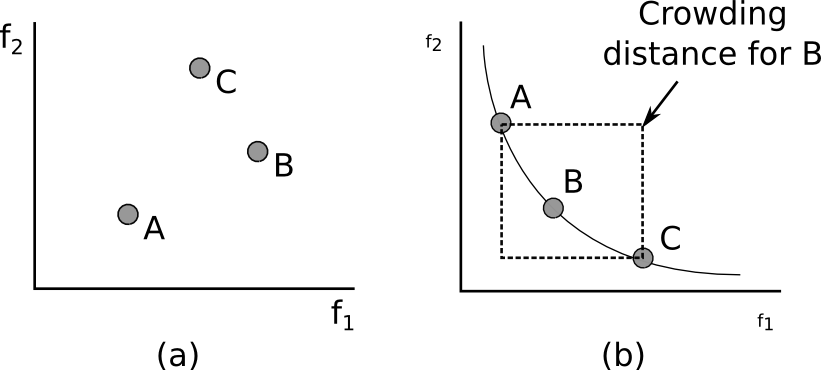
\includegraphics[width=110mm,natwidth=821,natheight=370]{bioinsp-rank-crowdingdist.png}
  \caption{Ranking and crowding distance: (a) A has rank 0, B and C rank 1, (b) crowding distance of solution B}
  \label{fig:rank-crowdingdist}
\end{figure}

\subsection{Particle swarm optimization}
The particle swarm optimization algorithm (PSO) mimics the behavior of a flock of birds. The birds in a flock usually follow a highlighted bird, for example the first one. If the highlighted bird changes its direction, the other birds will also adjust their direction. This principle can be used for optimization.

In PSO, the population consists of a number of particles (birds). Each particle has a position, a velocity and a fitness value. Each particle knows about the global best solution found so far (gBest), and its personal best solution (pBest), found so far. A particle moves in the direction of gBest and pBest. For this, in each iteration the particle adjusts its velocity according to its current velocity and the distance to gBest and pBest. Then it moves according to the adjusted velocity. This simple behavior lets the particle converge towards gBest.

The PSO can be implemented using a simple vector operation, given in formula \eqref{eq:pso-speed}.

\begin{equation}\label{eq:pso-speed}
  v(t) = w * v(t - 1) + c_1 * r_1 * (pBest - x(t - 1)) + c_2 * r_2 * (gBest - x(t - 1))
\end{equation}

This vector operation is performed for each iteration on all particles. $v(t)$ is the velocity of the particle at time $t$, $v(t - 1)$ is the velocity in the previous iteration and $x(t - 1)$ defines the position of the particle, also in the previous iteration. $w$ is called the inertia weight and defines the influence of the current speed on the new velocity. The parameter $c_1$ is called the cognitive acceleration coefficient and defines how much the particle is influenced by its personal best solution. $c_2$ is called the social acceleration coefficient and defines how much the particle is influenced by the global best solution. The parameters $r_1$ and $r_2$ are random values between 0 and 1 and are used as a source of diversity.

After the particles velocity is computed, its current position is updated using formula \eqref{eq:pso-position}
\begin{equation}\label{eq:pso-position}
  x(t) = v(t) + x(t - 1)
\end{equation}

\begin{figure}[ht!]
  \centering
  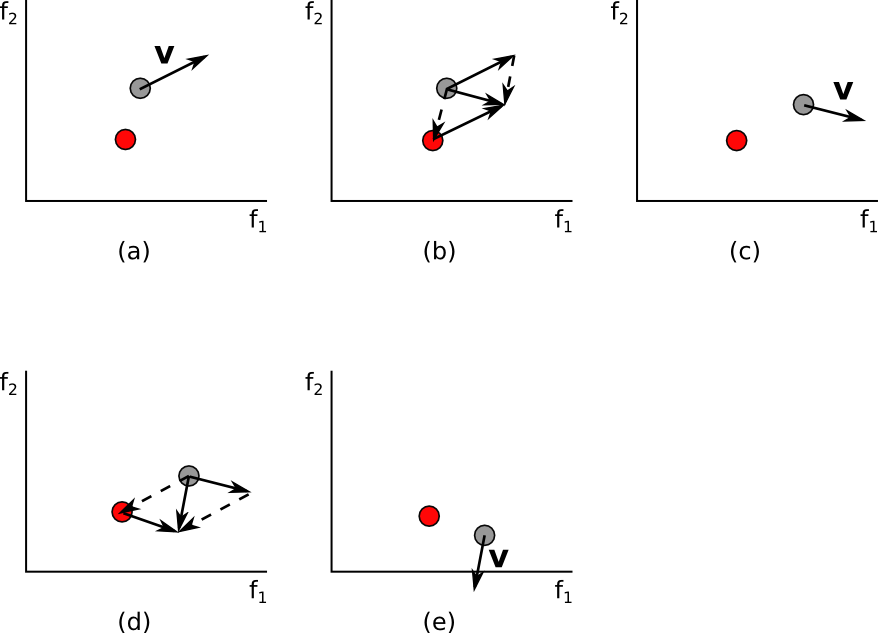
\includegraphics[width=130mm,natwidth=929,natheight=1037]{bioinsp-pso.png}
  \caption{Four iterations of PSO for a single particle. The red dot marks gBest, the gray dot the particle. The velocity and position of the particle does rely only on gBest in this example, pBest is not used}
  \label{fig:pso}
\end{figure}

An example of four iterations for a single particle can be found in figure \ref{fig:pso}. Figure \ref{fig:pso}(a) shows the initial situation, the red dot highlights gBest, the gray dot the particle. Figure \ref{fig:pso}(b) shows how the current velocity and position of the particle, as well as the position of gBest, influence the velocity and position of the particle in the next iteration, which is shown in figure \ref{fig:pso}(c). Figure \ref{fig:pso}(d) to \ref{fig:pso}(i) show additional iterations, all conforming to the same principle. The value of pBest is not considered in this example.

PSO can also be used to compute solutions to a MOP. In this case, the non-dominated solutions are stored in an archive. New solutions are inserted into the archive if they are non-dominated by the elements in the archive. Subsequently the archive is scanned for dominated solutions that can arise from new inserted solutions. The dominated solutions are removed from the archive. The non-dominated solutions to the MOP can be extracted from the archive after PSO terminates.

\section{Parallelization using the island model}
\label{chap:bioalgorithms:island-model}
The island model is a high level parallelization model that is sometimes used in optimization problems. In the island model, several optimization algorithms run in parallel, trying to compute the result to the same problem. The parallel running algorithms are called the islands. Each of these algorithms is independent of the others, and each one may have a different solution at a given point of time. By exchanging their data after some intervals, islands may get interesting solutions from other islands that can be integrated in their own computation to enhance their solution. If we take the GA as an example, the islands would consist of independently running GAs that exchange individuals to improve the solution. Figure \ref{fig:island-model} shows an example island model with 3 GAs that exchange individuals.

\begin{figure}[ht!]
  \centering
  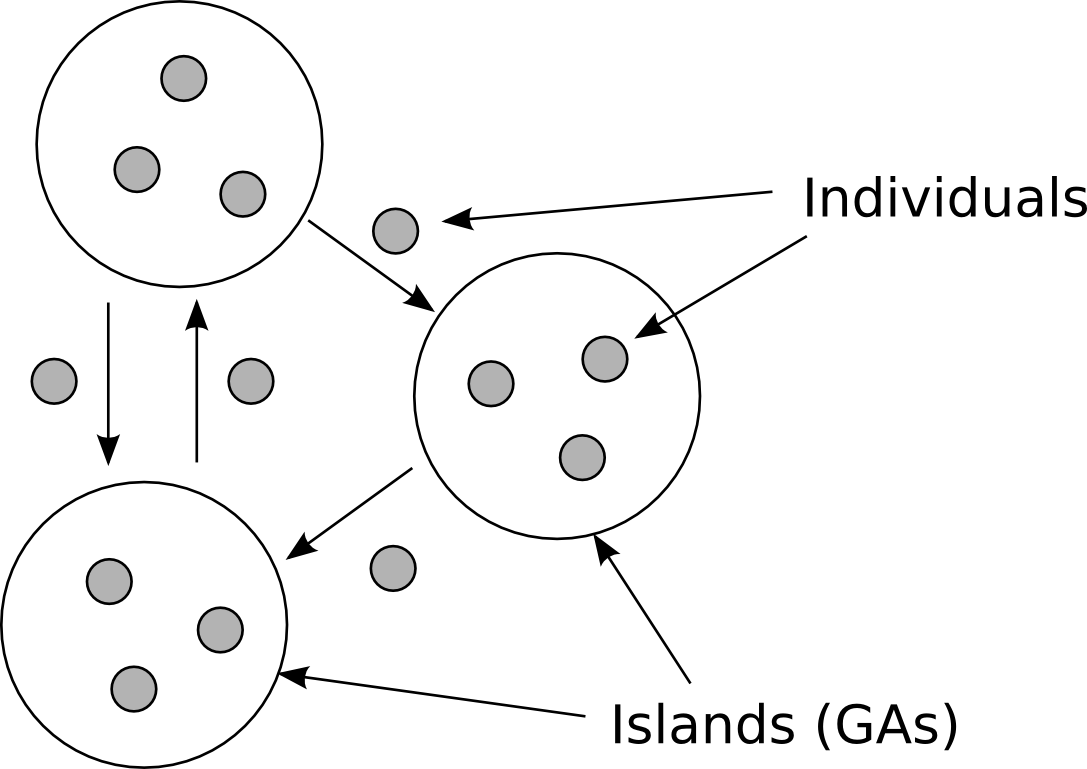
\includegraphics[width=70mm,natwidth=1087,natheight=769]{island-model.png}
  \caption{Example island model with 3 GAs, exchanging individuals}
  \label{fig:island-model}
\end{figure}

The island model enhances the exploratory behavior of optimization algorithms, which often results in better overall solutions. As the data exchange is only done at certain points of time, the islands have the chance to exploit their own solution. When they get stuck in a local optima, they get the chance to escape this optima by considering solutions from other islands.

Biohadoop, the framework implemented during this thesis, provides the capabilities to execute an island model. More information can be found in \ref{chap:impl:island-model}.

% \subsection{Ant colony optimization}
% The ant colony optimization (ACO) is an optimization technique for combinatorial problems, like the TSP. It is inspired by ant colonies, that are very effective in finding shortest paths from their nest to a source of food.
% 
% To find this paths, ants deposit a pheromone on the track they are using. The pheromone evaporates over time, such that paths that are frequently used (for example because they are shorter), have more pheromones applied, than seldom used paths. If an ant must decide which path to take, it follows with a higher probability the path that has the most pheromones applied. While using this path, it applies again pheromones, which increases the probability that other ants will follow this path.
% 
% Individually, the ants take only simple decisions, based on the amount of pheromones on a given path. Collectively, they work on solving an optimization problem.